
\begin{frame}{MLE estimation}
    Define
    $
        f_\beta := (\beta_s I_s(t) + \beta_a I_a(t) ),
    $
    thus
    $$
        f_\beta-f_{\beta_0}
            =
            (\beta_s  -  \beta_{s,0}) I_s(t)
            +
            (\beta_a - \beta_{a,0}) I_a(t).
    $$
    With this notation we write
    \begin{align*}
        [ F(\mathbf{X}_{\beta,p}(t))  - F(\mathbf{X}_{\beta_0,p_0}(t)) ]
        &=
        \begin{pmatrix}
            -(f_\beta-f_{\beta_0}) \dfrac{S(t) }{\sigma (1-S(t))}
            \\
            -(f_\beta-f_{\beta_0}) \dfrac{S(t) }{\sigma E(t)}
            \\
            -(p - p_0) \dfrac{\kappa E(t)}{\sigma I_a(t)}
            \\
            (p-p_0) \dfrac{\kappa E(t)}{\sigma I_s(t)}
            \\
            0
        \end{pmatrix},
    \end{align*}
\end{frame}
%-------------------------------------------------------------------------------
\begin{frame}
    Then we obtain the likelihood (Radon-Nikodyn derivative)
    \begin{equation*}
        \label{Likelihood}
        \begin{aligned}
            \frac{d\mathbb{P}_\beta}{d\mathbb{P}_{\beta_0}}
            =&
            \exp
                \Bigg[ 
                    \int_0^T [ 
                        F(\mathbf{X}_{\beta,p}(t))  
                        -
                        F(\mathbf{X}_{\beta_0,p_0}(t)) ]^{T} 
                        Q^{-1} 
                        d\mathbf{W}(t)
            \\
            &-\frac{1}{2}
            \int_0^T  [ F(\mathbf{X}_{\beta,p}(t))  -
            F(\mathbf{X}_{\beta_0,p_0}(t)) ]^{T}Q^{-1}
            [ F(\mathbf{X}_{\beta,p}(t))  -
            F(\mathbf{X}_{\beta_0,p_0}(t)) ] d(t)\Bigg],
          \\
            f_\beta &=
                (\beta_s I_s(t) + \beta_a I_a(t))
          \\
            [
                F(\mathbf{X}_{\beta,p}(t)) -
                &
                F(\mathbf{X}_{\beta_0,p_0}(t)) ]
            =
            \begin{pmatrix}
                -(f_\beta-f_{\beta_0}) \dfrac{S(t) }{\sigma (1-S(t))}
                \\
                -(f_\beta-f_{\beta_0}) \dfrac{S(t) }{\sigma E(t)}
                \\
                -(p - p_0) \dfrac{\kappa E(t)}{\sigma I_a(t)}
                \\
                (p-p_0) \dfrac{\kappa E(t)}{\sigma I_s(t)}
                \\
                0
            \end{pmatrix}, \qquad \mathbb{Q} = \mathbb{I}_5 \text{  (identity)}
        \end{aligned}
    \end{equation*}
    Therefore we can estimate $\widehat{\varphi} = (\beta_s, \beta_a, p)$ by
    maximizing
    $-\log(\text{likelihood})$.
\end{frame}
%-------------------------------------------------------------------------------
\begin{frame}{}
    For exmple, to estimte $p$, we derive the $-\log(\text{likelihood})$ with
    respect to $p$ and deduce an expresion to find a extrema.
    \begin{align*}
        (p-p_0)
        &
        \underbrace{%
            \left(
                \int_0^T
                \Big[
                    \dfrac{\kappa^2 E^2(t)}{ I_s^2(t)}
                    + \dfrac{\kappa^2 E^2(t)}{ I_a^2(t)}
                \Big] dt
            \right)
        }_{:=J_2(T)}
        -
        \sigma
            \int_0^T
            \Big[
                -\dfrac{\kappa E(t)}{ I_a(t)} +
                \dfrac{\kappa E(t)}{ I_s(t)}
            \Big] dW(t) = 0
        \\
        \\
        \hat{p}_{ML}-p_0 &=
            \frac{\sigma }{J_2(T)}
            \int_0^T
                \Big[
                    - \dfrac{\kappa E(t)}{ I_a(t)}
                    + \dfrac{\kappa E(t)}{ I_s(t)}
                \Big] dW(t),
    \end{align*}
\end{frame}

\begin{frame}{Estimator consistency}
    Let
    $
    X_0 ^ + :=
    \{
        (
        S(t_0),
        E(t_0),
        I_a(t_0),
        I_s(t_0)
        )
    \}
    $ initial state where all populations classes are strictly positive. Denote
    by
    $
    \varphi:=
    \left\{
    \mu,
    \beta_s,
    \beta_a,
    \kappa,
    p ,
    \theta,
    \alpha_s ,
    \alpha_a,
    \gamma
    \right\},
    $
    a model parameter configuration.  The reproductive number
    for the deterministic version $(\sigma=0)$
    $$
    \mathcal{R}_0^{D}:=
    \dfrac{p \kappa \beta_s }{(\mu + \kappa) (\mu + \alpha_s)}
    +
    \dfrac{(1 - p) \kappa \beta_a}{(\mu + \kappa)(\mu + \alpha_a)}.
    $$
    Define
    \begin{equation*}
        \begin{aligned}
            \Omega^{*} :=
            \left \{
            (S, E, I_a, I_s, R) \times [t_0 , T]:
            \right.
            &
            S(T) \leq S(t) < S(t_0),
            \\
            &
            \left.
            E(t) > E(t_0), \
            I_a(t) > I_a(t_0), \
            I_s(t) > I_s(t_0)
            \right \}.
        \end{aligned}
    \end{equation*}
    \begin{theorem}
        Let $T_0>0$ such that for all $t\in[0, T_0]$
        \begin{enumerate}[label = \roman*.]
            \item The deterministic threshold $\mathcal{R}_0^D >1$
            \item The initial condition $X_0^+$ and parameters configuration
                $\varphi$ are such that $\Omega ^ * \neq \emptyset$
        \end{enumerate}
            Then, the estimators
        $(\hat{\beta}_{s,ML},\hat{\beta}_{a,ML},\hat{p}_{ML})$
        are  strongly consistent, that is,
        \begin{equation*}
            \label{consistency}
            \lim_{T \rightarrow T_0}
            \begin{pmatrix}
                \hat \beta_{s,ML}
                \\
                \hat \beta_{a,ML}
                \\
                \hat p_{ML}
            \end{pmatrix}
            =
            \begin{pmatrix}
                \beta_{s,0}
                \\
                \beta_{a,0}
                \\
                p_0
            \end{pmatrix},
            \qquad \mbox{w.p.1.}
        \end{equation*}
    \end{theorem}
\end{frame}
\begin{frame}{To estimate the parameter of diffusion $\sigma$}
    To estimate the parameter of diffusion $\sigma$,
    we use the quadratic variation over $[0,T]$,  $<*,*>_T$,
    of the solution processes
    \begin{equation*}\label{est_sigma}
        \hat{\sigma}^2:=\sum_{i=1}^5\frac{\hat{\sigma}^2_i}{5},
    \end{equation*}
    where
    \begin{equation*}
        \label{sigmas}
        \begin{aligned}
            &\hat{\sigma}^2_1
            = \frac{<S,S>_T}{\int_0^T(1-S(t))^2dt},
            %
            \qquad
            \hat{\sigma}^2_2
            = \frac{<E,E>_T}{\int_0^TE(t)^2dt},
            % %
            \qquad
            \hat{\sigma}^2_3
            = \frac{<I_a,I_a>_T}{\int_0^TI_a(t)^2dt},
            % %
            \\
            & \hat{\sigma}^2_4
            = \frac{<I_s,I_s>_T}{\int_0^TI_s(t)^2dt},
            % %
            \qquad
            \hat{\sigma}^2_5
            = \frac{<R,R>_T}{\int_0^TR(t)^2dt}.
        \end{aligned}
    \end{equation*}
\end{frame}
%--------------------------------------------------------------------------------
\begin{frame}
    \begin{algorithm}[H]
        \begin{algorithmic}[1]
            \STATE
                Fix
                $E(0),I_a(0)$ and $R(0)$,
                $S(0)=1-E(0)-I_a(0) -R(0)-I^{mx}_s$, and make $n=0$.
            \STATE
                Generate $\Delta W\sim N(0,\Delta)$.
            \STATE
                \begin{equation*}
                    \begin{aligned}
                        S(t_{n+1}) = &
                            S(t_n) +
                            [
                                \mu + \gamma R(t_n)
                                -(
                                    \mu + \beta_a I_a(t_{n})
                                        + \beta_s
                                        \textcolor{orange}{
                                            I_s ^{mx}(t_n)
                                        }
                                 ) S(t_{n})
                            ] \Delta
                            \\
                            & + \sigma(1 - S(t_n)) \Delta W
                        \\
                        E(t_{n+1}) = &
                            E(t_{n})
                            +
                            [
                                (
                                    \beta_a I_a (t_{n})
                                    +
                                    \beta_s
                                    \textcolor{orange}{
                                        I_s ^ {mx}(t_n)
                                    }
                                ) S(t_{n})
                            - (\kappa + \mu) E(t_{n})
                            ] \Delta
                            \\
                            &-
                            \sigma (E(t_n)) \Delta W
                        \\
                        I_a(t_{n+1}) &=
                            I_a(t_{n})
                          + (
                                p \kappa E(t_{n})
                                - \alpha_a+\mu) I_a(t_{n}
                            ) \Delta
                            -\sigma I_a(t_{n}) \Delta w
                        \\
                        R(t_{n+1})
                            &=
                            1 - S(t_{n+1}
                              -E(t_{n+1})
                              -I_a(t_{n+1})
                              -\textcolor{orange}{I^{mx}_s(t_{n+1})}
                    \end{aligned}
               \end{equation*}
        \end{algorithmic}
        \caption{
            Approximation by Euler-Mayurama.
            $\textcolor{orange}{I^{mx}_s (t_n)}$
            observation data.
        }
    \end{algorithm}
\end{frame}
%-------------------------------------------------------------------------------
\begin{frame}{Simulation}
        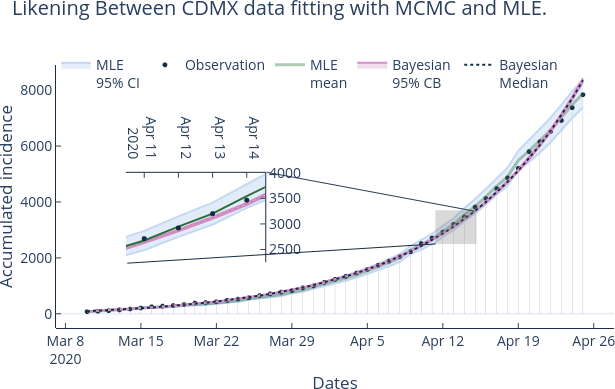
\includegraphics[width=\linewidth]{sto_mle_covid19/Figures/Likening.png}
\end{frame}
